

\tikzset{every picture/.style={line width=0.75pt}} %set default line width to 0.75pt        

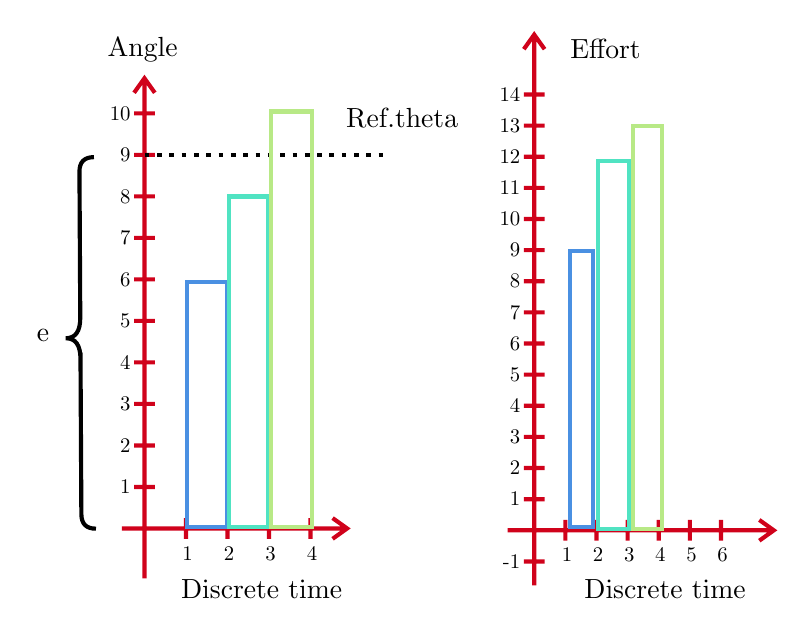
\begin{tikzpicture}[x=0.75pt,y=0.75pt,yscale=-1,xscale=1]
%uncomment if require: \path (0,530); %set diagram left start at 0, and has height of 530

%Shape: Axis 2D [id:dp6346571706526563] 
\draw [color={rgb, 255:red, 208; green, 2; blue, 27 }  ,draw opacity=1 ][line width=1.5]  (86,259.9) -- (194.5,259.9)(96.85,43) -- (96.85,284) (187.5,254.9) -- (194.5,259.9) -- (187.5,264.9) (91.85,50) -- (96.85,43) -- (101.85,50) (116.85,254.9) -- (116.85,264.9)(136.85,254.9) -- (136.85,264.9)(156.85,254.9) -- (156.85,264.9)(176.85,254.9) -- (176.85,264.9)(91.85,239.9) -- (101.85,239.9)(91.85,219.9) -- (101.85,219.9)(91.85,199.9) -- (101.85,199.9)(91.85,179.9) -- (101.85,179.9)(91.85,159.9) -- (101.85,159.9)(91.85,139.9) -- (101.85,139.9)(91.85,119.9) -- (101.85,119.9)(91.85,99.9) -- (101.85,99.9)(91.85,79.9) -- (101.85,79.9)(91.85,59.9) -- (101.85,59.9) ;
\draw   (123.85,271.9) node[anchor=east, scale=0.75]{1} (143.85,271.9) node[anchor=east, scale=0.75]{2} (163.85,271.9) node[anchor=east, scale=0.75]{3} (183.85,271.9) node[anchor=east, scale=0.75]{4} (93.85,239.9) node[anchor=east, scale=0.75]{1} (93.85,219.9) node[anchor=east, scale=0.75]{2} (93.85,199.9) node[anchor=east, scale=0.75]{3} (93.85,179.9) node[anchor=east, scale=0.75]{4} (93.85,159.9) node[anchor=east, scale=0.75]{5} (93.85,139.9) node[anchor=east, scale=0.75]{6} (93.85,119.9) node[anchor=east, scale=0.75]{7} (93.85,99.9) node[anchor=east, scale=0.75]{8} (93.85,79.9) node[anchor=east, scale=0.75]{9} (93.85,59.9) node[anchor=east, scale=0.75]{10} ;
%Straight Lines [id:da8395435041805068] 
\draw [line width=1.5]  [dash pattern={on 1.69pt off 2.76pt}]  (97,80) -- (214.5,80) ;


%Shape: Brace [id:dp15804314182279944] 
\draw  [line width=1.5]  (72.5,81) .. controls (67.83,81.03) and (65.51,83.37) .. (65.54,88.04) -- (65.93,158.23) .. controls (65.97,164.9) and (63.66,168.24) .. (58.99,168.27) .. controls (63.66,168.24) and (66.01,171.56) .. (66.04,178.23)(66.03,175.23) -- (66.46,253.04) .. controls (66.49,257.71) and (68.83,260.03) .. (73.5,260) ;
%Shape: Rectangle [id:dp5191693992255162] 
\draw  [color={rgb, 255:red, 74; green, 144; blue, 226 }  ,draw opacity=1 ][line width=1.5]  (117.5,141) -- (136.5,141) -- (136.5,259) -- (117.5,259) -- cycle ;
%Shape: Rectangle [id:dp2287664558829514] 
\draw  [color={rgb, 255:red, 80; green, 227; blue, 194 }  ,draw opacity=1 ][line width=1.5]  (137.67,100) -- (156.5,100) -- (156.5,259) -- (137.67,259) -- cycle ;
%Shape: Rectangle [id:dp3261576138135398] 
\draw  [color={rgb, 255:red, 184; green, 233; blue, 134 }  ,draw opacity=1 ][line width=1.5]  (157.67,59) -- (177.67,59) -- (177.67,259) -- (157.67,259) -- cycle ;
%Shape: Axis 2D [id:dp473563119637739] 
\draw [color={rgb, 255:red, 208; green, 2; blue, 27 }  ,draw opacity=1 ][line width=1.5]  (271.82,260.8) -- (400.08,260.8)(284.64,22) -- (284.64,287.33) (393.08,255.8) -- (400.08,260.8) -- (393.08,265.8) (279.64,29) -- (284.64,22) -- (289.64,29) (299.64,255.8) -- (299.64,265.8)(314.64,255.8) -- (314.64,265.8)(329.64,255.8) -- (329.64,265.8)(344.64,255.8) -- (344.64,265.8)(359.64,255.8) -- (359.64,265.8)(374.64,255.8) -- (374.64,265.8)(279.64,245.8) -- (289.64,245.8)(279.64,230.8) -- (289.64,230.8)(279.64,215.8) -- (289.64,215.8)(279.64,200.8) -- (289.64,200.8)(279.64,185.8) -- (289.64,185.8)(279.64,170.8) -- (289.64,170.8)(279.64,155.8) -- (289.64,155.8)(279.64,140.8) -- (289.64,140.8)(279.64,125.8) -- (289.64,125.8)(279.64,110.8) -- (289.64,110.8)(279.64,95.8) -- (289.64,95.8)(279.64,80.8) -- (289.64,80.8)(279.64,65.8) -- (289.64,65.8)(279.64,50.8) -- (289.64,50.8)(279.64,275.8) -- (289.64,275.8) ;
\draw   (306.64,272.8) node[anchor=east, scale=0.75]{1} (321.64,272.8) node[anchor=east, scale=0.75]{2} (336.64,272.8) node[anchor=east, scale=0.75]{3} (351.64,272.8) node[anchor=east, scale=0.75]{4} (366.64,272.8) node[anchor=east, scale=0.75]{5} (381.64,272.8) node[anchor=east, scale=0.75]{6} (281.64,245.8) node[anchor=east, scale=0.75]{1} (281.64,230.8) node[anchor=east, scale=0.75]{2} (281.64,215.8) node[anchor=east, scale=0.75]{3} (281.64,200.8) node[anchor=east, scale=0.75]{4} (281.64,185.8) node[anchor=east, scale=0.75]{5} (281.64,170.8) node[anchor=east, scale=0.75]{6} (281.64,155.8) node[anchor=east, scale=0.75]{7} (281.64,140.8) node[anchor=east, scale=0.75]{8} (281.64,125.8) node[anchor=east, scale=0.75]{9} (281.64,110.8) node[anchor=east, scale=0.75]{10} (281.64,95.8) node[anchor=east, scale=0.75]{11} (281.64,80.8) node[anchor=east, scale=0.75]{12} (281.64,65.8) node[anchor=east, scale=0.75]{13} (281.64,50.8) node[anchor=east, scale=0.75]{14} (281.64,275.8) node[anchor=east, scale=0.75]{-1} ;
%Shape: Rectangle [id:dp06820965849131166] 
\draw  [color={rgb, 255:red, 74; green, 144; blue, 226 }  ,draw opacity=1 ][line width=1.5]  (301.75,126.33) -- (313.08,126.33) -- (313.08,259) -- (301.75,259) -- cycle ;
%Shape: Rectangle [id:dp16997023555555235] 
\draw  [color={rgb, 255:red, 80; green, 227; blue, 194 }  ,draw opacity=1 ][line width=1.5]  (315.5,82.67) -- (330.5,82.67) -- (330.5,260) -- (315.5,260) -- cycle ;
%Shape: Rectangle [id:dp21980087841289575] 
\draw  [color={rgb, 255:red, 184; green, 233; blue, 134 }  ,draw opacity=1 ][line width=1.5]  (332.08,66) -- (346.08,66) -- (346.08,260) -- (332.08,260) -- cycle ;

% Text Node
\draw (221,62.33) node  [align=left] {Ref.theta};
% Text Node
\draw (48,167) node  [align=left] {e};
% Text Node
\draw (96,29) node  [align=left] {Angle};
% Text Node
\draw (153.33,289) node  [align=left] {Discrete time};
% Text Node
\draw (319,29) node  [align=left] {Effort};
% Text Node
\draw (347.67,289.33) node  [align=left] {Discrete time};


\end{tikzpicture}